%================================================================
\section{Results}\label{sec:results}
% Present results and give a critical discussion of my work in 
% the context of other work. Relate the work to previous studies, 
% and make sure the results are reproducible. Include information 
% in figure captions such that they can give the reader enough to 
% understand the main gist of the report.
%================================================================
Method? Data from a grid of $100 \times 100$ data points. For each polynomial degree up to 5, I created the corresponding design matrix, and split the input and target data into train and test set.

I generated data from the franke function, both with and without stochastic noise, and performed an OLS regression analysis up to polynomial of degree 5. I computed the MSE and R$^{2}$-score for predictions on both data set, the result is shown in Figure \ref{fig:ols_error} and Figure \ref{fig:ols_error_noisy}, respectively.
\begin{figure}
    \centering
    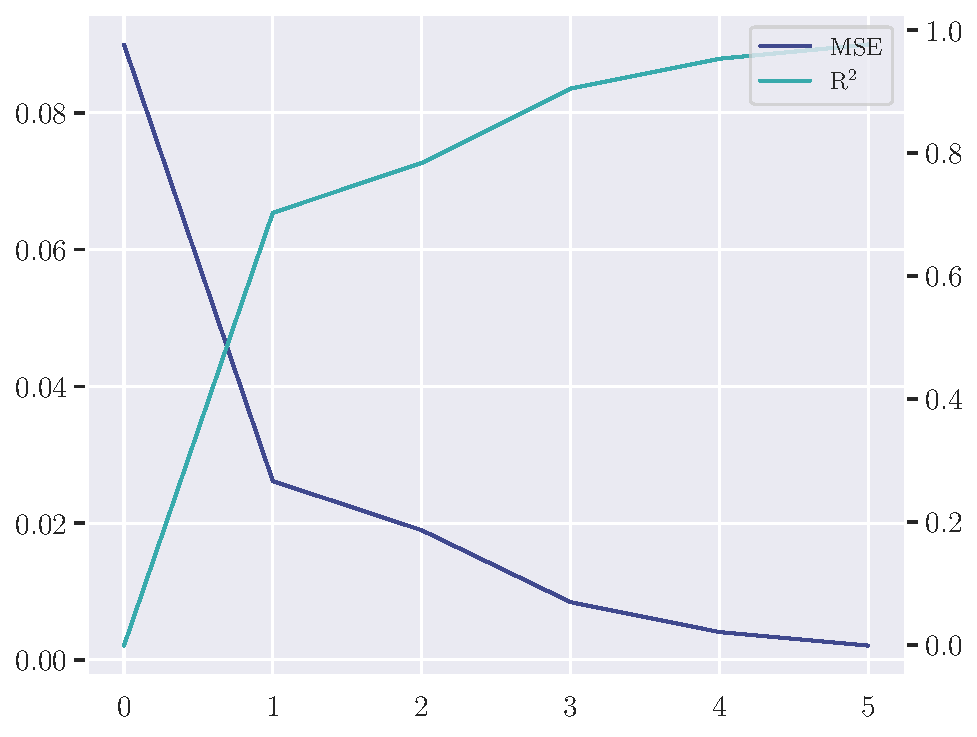
\includegraphics[width=0.8\linewidth]{project-1/latex/figures/ols_error.pdf}
    \caption{MSE and R$^{2}$-score computed on test data, as a function of the polynomial degree of the input features. The function data was generated without stochastic noise.}
    \label{fig:ols_error}
\end{figure}

\begin{figure}
    \centering
    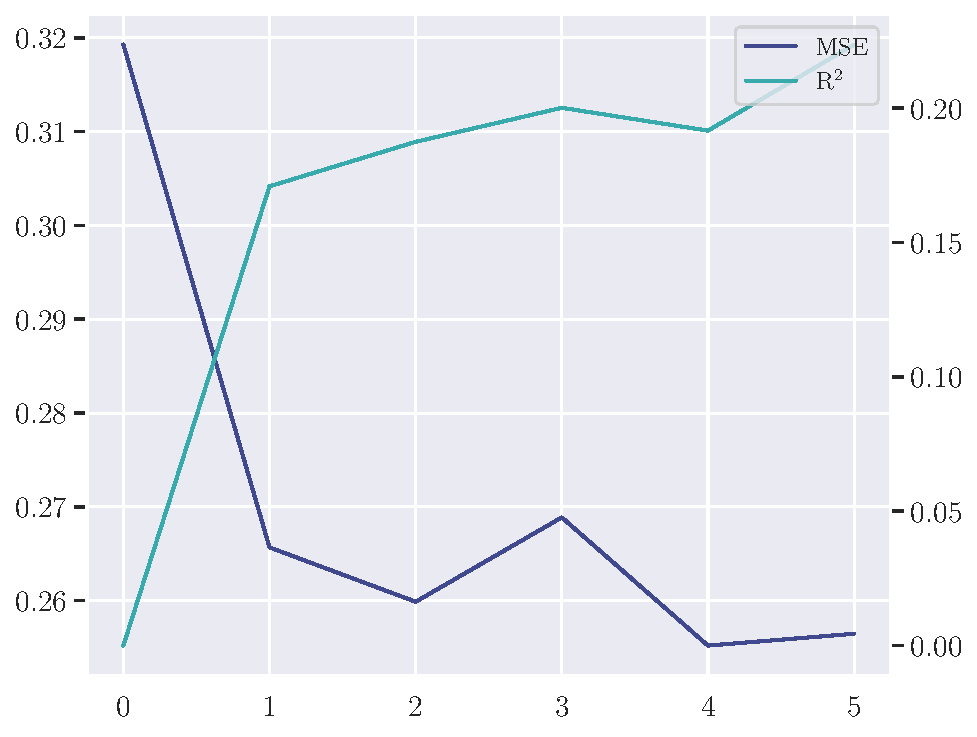
\includegraphics[width=0.8\linewidth]{project-1/latex/figures/ols_error_noisy.pdf}
    \caption{MSE and R$^{2}$-score computed on test data, as a function of the polynomial degree of the input features. The function data includes stochastic noise $\epsilon \in \mathcal{N}(0, 1)$.}
    \label{fig:ols_error_noisy}
\end{figure}

Calculate MSE and R2 for each prediction, using the test data.

The MSE and R2-score for the franke function without noise is shown in Figure (), and including noise in Figure (). The error decreases as the polynomial degree increases, this is more apparent when comparing the prediction of the noiseless function. When the maximum polynomial degree is set to 15, the test error reach a minima around degree (). While the training error continue to decrease, the test error increase for higher polynomial order, often seen when the model is overfitting to the training data.

For ridge